\documentclass[xcolor={usenames,dvipsnames,svgnames}, compress]{beamer}

% \usepackage[utf8]{inputenc}
\usepackage{booktabs}
\usepackage{dcolumn}
\usepackage{colortbl}
\usepackage{hyperref}

% \usepackage[style=authoryear-comp, backref=true]{biblatex}
\usepackage{ifxetex}
\usepackage{amsmath}
\usepackage{biblatex}
% 
\usepackage[no-math]{fontspec}

% 
% CLIPS listings
%\usepackage[utf8]{inputenc}
\usepackage{listings}
\usepackage{xcolor}


%
% I asked on stackoverflow for rainbow parentheses
% http://tex.stackexchange.com/questions/235740/rainbow-parentheses-in-lisp-listings
% the palette is from solarized theme
\definecolor{solarized-cyan}{RGB}{42, 161, 152}
\definecolor{solarized-magenta}{RGB}{211, 54, 130}
\definecolor{solarized-yellow}{RGB}{181, 137, 0}
\definecolor{solarized-violet}{RGB}{108, 113, 196}
\definecolor{solarized-red}{RGB}{220, 50, 47}
\definecolor{solarized-orange}{RGB}{203, 75, 22}
\definecolor{solarized-grey}{RGB}{101, 123, 131}

\lstdefinelanguage{clips}
{
  classoffset=0,
  morekeywords ={deffunction, deftemplate, defglobal, defmodule, defrule, deffacts, nil, assert, retract},
  keywordstyle=\bfseries\color{solarized-orange},
  classoffset=1,
  morekeywords ={delcare, salience, run, slot, multislot, clear, reset, facts, exit, agenda, initial-fact, watch, ppdefrule, unwatch, printout, if, then, else, while, loop-count, crlf, read, readline},
  keywordstyle=\bfseries,
  %classoffset=2,
  %keywordsprefix=\?,
  %alsoletter=\?,
  %keywordstyle=\itshape\color{solarized-red},
  classoffset=0,
  sensitive=true,
  morecomment=[l]{;},
  morestring=[b]{"},
  stringstyle=\color{solarized-grey},
  basicstyle=\scriptsize,%\ttfamily\scriptsize,
  numbers=left,
  numbersep=-5pt,
  numberstyle=\tiny,
  showstringspaces=false,
  }

\renewcommand{\ttdefault}{pcr}

% egreg's modulo macro (see http://tex.stackexchange.com/a/34449/21891)
\def\truncdiv#1#2{((#1-(#2-1)/2)/#2)}
\def\moduloop#1#2{(#1-\truncdiv{#1}{#2}*#2)}
\def\modulo#1#2{\number\numexpr\moduloop{#1}{#2}\relax}    

\makeatletter

% a TeX counter to keep track of the nesting level
\newcount\netParensCount@clisp

% Modify how ( and ) get typeset depending on the value of the counter
% (Based on Ulrike Fischer's approach to modifying characters in listings;
% see http://tex.stackexchange.com/a/231927/21891)
\lst@CCPutMacro
\lst@ProcessOther{`(}{{%
    \ifnum\lst@mode=\lst@Pmode\relax%
    \rainbow@clisp{(}%
    \global\advance\netParensCount@clisp by \@ne%
    \else
    (%
    \fi
  }}%
\lst@ProcessOther{`)}{{%
    \ifnum\lst@mode=\lst@Pmode\relax%
    \global\advance\netParensCount@clisp by \m@ne%
    \rainbow@clisp{)}%
    \else
    )%
    \fi
  }}%
\@empty\z@\@empty
% Color its argument based on the value of the \netParensCount@clisp counter
% (modulo 5)
\newcommand\rainbow@clisp[1]{%
  \ifcase\modulo\netParensCount@clisp 5\relax%
  \textcolor{solarized-cyan}{\bfseries#1}%
  \or
  \textcolor{solarized-yellow}{\bfseries#1}%
  \or
  \textcolor{solarized-magenta}{\bfseries#1}%
  \or
  \textcolor{solarized-violet}{\bfseries#1}%
  \else
  \textcolor{solarized-red}{\bfseries#1}%
  \fi
}

% Alternatively, you could simplify the definition of \rainbow@clisp to...
% \newcommand\rainbow@clisp[1]{%
% \textcolor{color\modulo\netParensCount@clisp 5}{#1}%
% }
%   ... but this assumes that the colours have names of the form color<i>,
%   where <i> is a positive integer

%   reset the counter at the beginning of each listing
%   (just in case there were unmatched parentheses in a previous listing)
\lst@AddToHook{PreInit}{%
  \global\netParensCount@clisp 0\relax%
}

\makeatother




\lstnewenvironment{clips-code}[1][]
{\lstset{language=clips,
    #1
  }}
{}






%%% Local Variables:
%%% mode: latex
%%% TeX-master: t
%%% End:


\definecolor{jess-fucsia}{RGB}{170, 0, 127}


\hypersetup{
  colorlinks=true,       % false: boxed links; true: colored links
  linkcolor=jess-fucsia,          % color of internal links (change box color with linkbordercolor)
  % citecolor=green,        % color of links to bibliography
  %filecolor=magenta,      % color of file links
  urlcolor=jess-fucsia           % color of external links
}

%%% Local Variables:
%%% mode: latex
%%% TeX-master: t
%%% End:




\usepackage{lacamlisciotheme/beamerthemelacamliscio}


% 
% customizing itemize items
% \setbeamertemplate{itemize item}{\textbf{\unichar{"2295}}}
% \setbeamertemplate{itemize item}{\raise .4ex\hbox{\tiny\textcolor{lacamlilac}{$\boldsymbol{\oplus}$}}\hspace{-2pt}}
% \setbeamertemplate{itemize subitem}{\raise .2ex\hbox{\tiny\textcolor{lacamlilac}{$\boldsymbol{\otimes}$}}\hspace{-2pt}}
% \setbeamertemplate{itemize subsubitem}{\textcolor{lacamlilac}{$\oplus$}}
% \setbeamertemplate{bibliography item}{\hspace{10pt}\raise .2ex\hbox{\tiny\textcolor{lacamlilac}{$\boldsymbol{\oplus}$}}}


% \addbibresource{../referomnia/referomnia.bib}

\setbeamertemplate{headline}{}

%%%%%%%%%%%%%%%%%%%%%%%%%%%%%%%%%%%%%%%%%%%%%%%%%%%%%%%%%%%% 
%%%%%%%%%%%%%%%%%%%%%%%%%%%%%%%%%%%%%%%%%%%%%%%%%%%%%%%%%%%% 
%%%%%%%%%%%%%%%%%%%%%%%%%%%%%%%%%%%%%%%%%%%%%%%%%%%%%%%%%%%% 


\begin{document}

% \title{Metodi di Apprendimento Statistico-Relazionale: Sum-Product Network \& Co-clustering}
\title{CLIPS:  (Advanced) Pattern Matching \& Functional Abstraction}
%\subtitle{An Introduction}
\author{Antonio Vergari}
% \institute{Lacam$@$DIB$@$Uniba}
\institute{Università degli Studi di Bari}
\department{Dipartimento di Informatica}
\laboratory{LACAM}
\group{Machine Learning}
\institutelogo{
\includegraphics[width=25pt]{Figures/unibaba}}
\lablogo{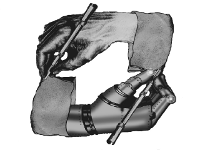
\includegraphics[width=35pt]{Figures/lacam}}

\footnotesize \let\small\footnotesize





{
  \setbeamertemplate{headline}{}
  \setbeamertemplate{footline}{}
  \begin{frame}
    \titlepage
  \end{frame}
}





\section{(Advanced) Pattern Matching}
{\setbeamertemplate{headline}{}
  \begin{frame}
    \sectionpage
  \end{frame}
}

\begin{frame}[fragile]
  \frametitle{Variables and Wildcards}
  As already seen we can use $?$ and $\$?$ to represent variables for
  single or multifields in rules. They are called \emph{wildcards} in CLIPS.
  \begin{clips-code}[numbers=none]
    (defrule move-to-floor
        ?goal <- (goal (move ?block1) (on-top-of floor))
        ?stack-1 <- (stack ?block1 $?rest)
        =>
        (retract ?goal ?stack-1)
        (assert (stack ?block1))
        (assert (stack $?rest))
        (printout t ?block1 " moved on top of floor." crlf))    
      \end{clips-code}

  When it is not necessary to bind variable names across multiple patters
  or functions, one can use anonymous wildcards:
  \begin{clips-code}[numbers=none]
    (defrule is-parent ;; family_dag_template.clp
        "asserting parenthood"
        (person (name ?name) (gender ?) (children $?))
        =>
        (assert (is-parent (name ?name))) ;; no need for $? or ? 
  \end{clips-code}
\end{frame}

\begin{frame}[fragile]
  \frametitle{Field Constraints I}
  Rules as advanced queries can specify constraints to the referred
  field values in a LHS pattern.\par
  Imagine this \textsf{deftemplate} to conceptualize a bit of
  knowledge about films:
  \begin{clips-code}[numbers=none]
    (deftemplate movie
        (slot title (type STRING) (default ?NONE))
        (slot genre (type SYMBOL)
            (allowed-symbols noir romance action cartoon indie surreal))
        (slot main-actor (type STRING))
        (multislot actors (type STRING))
        (slot director (type STRING))
        (slot producer (type STRING)))
  \end{clips-code}

  To express a query about film not belonging to a genre we can use
  the operator $\mathbf{\sim}$ (\emph{not}):
  \begin{clips-code}[numbers=none]
    (defrule interesting-movies
        "Defining interesting films as those not belonging to the romance genre"
        (movie (title ?title) (genre ~romance))
        =>
        (printout t "An interesting movie " ?title crlf))
  \end{clips-code}
\end{frame}

\begin{frame}[fragile]
  \frametitle{Field Constraints II}
  Similarly to the not constraint, one can express an or constraing,
  allowing a subset of values to make a field matchable. They can be separated by a pining $\mathbf{|}$:
  \begin{clips-code}[numbers=none]
    (defrule hipster-movies
        (movie (title ?title) (genre indie | surreal))
        =>
        (printout t "Probably an hipster movie " ?title crlf))    
  \end{clips-code}
  The alternative was to write two different rules:
  \begin{clips-code}[numbers=none]
    (defrule hipster-movies-I
        (movie (title ?title) (genre indie))
        =>
        (printout t "Probably an hipster movie " ?title crlf))

    (defrule hipster-movies-II
        (movie (title ?title) (genre surreal))
        =>
        (printout t "Probably an hipster movie " ?title crlf))
  \end{clips-code}
\end{frame}

\begin{frame}[fragile]
  \frametitle{Field Constraints III}
  The and field constraing, expressed with an ampersand \textbf{\&},
  allows for an arbitrary concatenation of field constrains on a field
  pattern:
  \begin{clips-code}[numbers=none]
    (defrule intellectual-movies
        (movie (title ?title) (genre ?genre&~romance&~action))
        =>
        (printout t "Likely a movie for intellectuals: ", ?title crlf))
  \end{clips-code}

  The and constraint can be used to express constraints involving
  other fields in different pattern values as well:
  \begin{clips-code}[numbers=none]
    (defrule uncle-fc ;; back to the family DAG example
        (parent ?grandparent ?father)
        ;; what happens if we do not put this constraint? 
        (parent ?grandparent ?uncle&~?father)
        (parent ?father ?child)
        (male ?uncle)
        =>
        (assert (uncle-fc ?uncle ?child)))
 \end{clips-code}
\end{frame}

\begin{frame}[fragile]
  \frametitle{Field Constraints IV}
  \framesubtitle{Predicate field constraint}
  In conjunction with the and operator \textbf{\&} one can specify a
  custom constraing in the form of a function predicate on the
  referred variable with \textbf{:},
  \begin{clips-code}[numbers=none]
    (defrule eddie-murphy-movies
        "Listing films with Eddie Murphy as actor"
        (movie (title ?title)
               ;; member$ tests if an elem is in a multifield 
               (actors $?actors&:(member$ "Eddie Murphy" $?actors)))
        =>
        (printout t "A film with Eddie Murphy: " ?title crlf))
  \end{clips-code}

  To get the titles of movies engrossing more than a threshold:
  \begin{clips-code}[numbers=none]
    (defrule blockbuster-movies
        (movie (title ?title) (box-office ?total&:(> ?total 500.0)))
        =>
        (printout t "Surely a blockbuster: " ?title crlf))
  \end{clips-code}
\end{frame}

% \begin{frame}
%   \frametitle{Return Value Field Constraint}
%   \framesubtitle{function returned values}
% \end{frame}

\begin{frame}[fragile]
  \frametitle{Test predicate}
  To introduce constraints in the LHS in a similar fashion we can employ the \textbf{test} predicate function. It
  evaluates the truth of a condition expressed by operators like \textbf{eq}, \textbf{neq}, \textbf{>},
  \textbf{<},\dots  Here it is another take on the rule for derive the uncle
  relationship:
  \begin{clips-code}[numbers=none]
    (defrule uncle
        (parent ?grandparent ?father) (parent ?grandparent ?uncle)
        (parent ?father ?child) (male ?uncle)
        (test (neq ?uncle ?father)) ;; a test predicate pattern
        (defrule hipster-movies-or
  ""
  (or (movie (title ?title) (genre indie))
      (movie (title ?title) (genre surreal)))
  
  =>
  (printout t "Probably an hipster movie (OR): " ?title crlf))=>
        (assert (uncle ?uncle ?child)))
  \end{clips-code}

  How to retrieve movies where the director is also the main actor and producer:
  \begin{clips-code}[numbers=none]
    (defrule homemade-movies
        (movie (title ?title) 
        (director ?director) (producer ?producer) (main-actor ?actor))
        (test (eq ?producer ?director ?actor))
        =>
        (printout t "This is a one made film: " ?title crlf))
  \end{clips-code}
\end{frame}

\begin{frame}[fragile]
  \frametitle{And/Or Conditional Elements}
  CLIPS automatically considers all the patterns in a LHS to be in a
  logical AND. An \textbf{or} CE specifies two or more patterns in
  disjunction. As for the or field constraint, it is a shortcut to
  write more compact rules.
  \begin{clips-code}[numbers=none]
    (defrule hipster-movies-or
        (or (movie (title ?title) (genre indie))
        (movie (title ?title) (genre surreal)))
        =>
        (printout t "Probably an hipster movie (OR): " ?title crlf))
  \end{clips-code}
\end{frame}

\begin{frame}[fragile]
  \frametitle{Not Conditional Element}
  It is possible to express a pattern as the absence of a fact in the
  WM via the \textbf{not} CE.\par
  To match the names of orphans in the family DAG one can write:
  \begin{clips-code}[numbers=none]
    (defrule orphan-2
         (or (male ?person)
             (female ?person))
         (or (not (father ?parent ?person))
             (not (mother ?parent ?person))
             (and
                 (not (father ?parent ?person))
                 (not (mother ?parent ?person))))
         =>
         (assert (orphan-2 ?person)))
       \end{clips-code}

       Be prepared to unexpected behaviors with the
       \href{http://en.wikipedia.org/wiki/Closed-world_assumption}{\emph{closed-world
           assumption}} (if something is not asserted in the WM is
       assumed to be false, e.g. if you do not generate some father
       and mother facts for all possible parenthood relationships, all
       persons will be considered orphans).    
\end{frame}

\begin{frame}[fragile]
  \frametitle{Exists Conditional Element}
  Similarly the \textbf{exists} CE checks for \emph{at least one fact
    in the WM} matching the
  referred pattern.\par\bigskip
  The difference with a simple pattern is that it
  generates only one rule activation.
  \begin{clips-code}[numbers=none]
    (defrule one-blockbuster
        "Check if there has been a movie surpassing 500"
        (exists (movie (box-office ?total&:(> ?total 500.0))))
        =>
        (printout t "There was one movie to engross > 500.0" crlf))
  \end{clips-code}
  It is implemented with a combination of and and not CE:
  \begin{clips-code}[numbers=none]
    (defrule one-blockbuster-I
        "Check if there has been a movie surpassing 500"
        (and (initial-fact)
            (not (not (movie (box-office ?total&:(> ?total 500.0))))))
            =>
            (printout t "There was one movie to engross > 500.0" crlf))
  \end{clips-code}
\end{frame}

\section{Functional Abstraction and Programming}
{\setbeamertemplate{headline}{}
  \begin{frame}
    \sectionpage
  \end{frame}
}

\begin{frame}
  \frametitle{The Game of Life}
  To explore a little bit of functional abstraction and programming in
  CLIPS we will use
  \href{http://en.wikipedia.org/wiki/Conway\%27s_Game_of_Life}{\textbf{Conway's
      Game of Life (GoL)}}. It is a formal system (\emph{cellular
    automaton}) in the form of a 2D finite grid in which cells can be alive
  (active) or dead (empty).\par
  The rules governing the evolution of the system are these two:
  \begin{enumerate}[I.]
  \item a live cell with exactly 2 or 3 live cells as neighbors lives, otherwise
    dies
  \item a dead cell with exactly 3 live cells as neighbors becomes alive
  \end{enumerate}

  The neighbors of a cell are the 8 adjacent cells surrounding
  it.\par\bigskip

  An example of a sequence of world statuses in a $5\times5$ grid is:
  \begin{table}
    \setlength\tabcolsep{2pt}
    \centering
    \tiny
    \begin{tabular}{c c c c c}
      
\includegraphics[width=40pt]{Figures/gol-osc-1}
      & 
\includegraphics[width=40pt]{Figures/gol-osc-2}
      & 
\includegraphics[width=40pt]{Figures/gol-osc-1}
      & 
\includegraphics[width=40pt]{Figures/gol-osc-2}
      & 
\includegraphics[width=40pt]{Figures/gol-osc-1}\\
      
      $t_0$ & $t_1$ & $t_2$& $t_3$ & $t_4$
    \end{tabular}
  \end{table}
\end{frame}

\begin{frame}[fragile]
  \frametitle{GoL I}
  \frametitle{A very simple conceptualization}
  If we want to implement GoL in CLIPS we shall represent the
  (current) \emph{world status} and the \emph{evolution rules}.\par\bigskip
  We will use an ordered facts of $N^2$ boolean values to represent a
  grid of $N\times N$ cells (what are the (dis)advantages?).\par
  The representation for the previous example at time $t_0$ is:
  \begin{clips-code}[numbers=none]
    (deffacts initial-world
        (world FALSE FALSE FALSE FALSE FALSE
               FALSE FALSE TRUE FALSE FALSE
               FALSE FALSE TRUE FALSE FALSE
               FALSE FALSE TRUE FALSE FALSE
               FALSE FALSE FALSE FALSE FALSE))
  \end{clips-code}

  We will model the evolutionary rules \emph{via user defined functions} this time, and use only
  one rule to update the current world status.           
\end{frame}



\begin{frame}[fragile]
  \frametitle{deffunction}
  CLIPS allows programmers to do functional abstraction and define
  their own functions with the \textsf{deffunction} construct:
  \begin{clips-code}[numbers=none]
    (deffunction <function-name>
        ?<optional-comment>
        (*<regular-parameter> ?<multifield-parameter>)
        *<action>)
  \end{clips-code}

  As in functional programming, the returned value is the last
  evaluated expression.\par
  Since we need to transform matrix coordinates
  into vectorial ones we could write:
  \begin{clips-code}[numbers=none]
    (deffunction vec-coords
        "Converts a pair of matrix coordinates into vector ones"
        (?x ?y ?width)
        (+ (* (- ?x 1) ?width) ?y))
  \end{clips-code}
\end{frame}



\begin{frame}[fragile]
  \frametitle{bind}
  To declare a variable with a local scope inside a function and
  initialize it to a value, one can use the \textsf{bind} function.
  \begin{clips-code}[numbers=none]
    (bind ?x 5)    (bind ?x (** 2 5))
  \end{clips-code}
  One could assign the value of an already defined variable as well:
  \begin{clips-code}[numbers=none]
    (bind ?x (* ?y ?x)) ;; x *= y
  \end{clips-code}
  Outside the scope in which bind is called the variable is undefined
  \begin{clips-code}
    CLIPS> (bind ?x (** 2 5))
    32.0
    CLIPS> (printout t ?x crlf)
    [EVALUATN1] Variable x is unbound
    CLIPS> (deffunction nth-pow-of-two (?n) (bind ?x (** 2 ?n)) ?x)
    CLIPS> (printout t ?x crlf)
    [EVALUATN1] Variable x is unbound
    CLIPS> (printout t (nth-pow-of-two 5) crlf)
    32.0
  \end{clips-code}
\end{frame}

\begin{frame}[fragile]
  \frametitle{Multifield functions I}
  Multifields represent the simplest data structure one can operate on
  in CLIPS: heterogeneous lists.\par
  Here are some useful functions on them:
  \textsf{create\$} initializes a list with the arguments provided.
  Passing no arguments results in the empty list.
  \begin{clips-code}
    CLIPS> (create$ hammer drill saw screw pliers wrench)
    (hammer drill saw screw pliers wrench)
    CLIPS> (create$ (+ 3 4) (* 2 3) (/ 8 4))
    (7 6 2.0)
  \end{clips-code}\bigskip
  
  \textsf{member\$} returns a the first position of the
  first argument if it appears in the multifield passed as the second
  argument, FALSE otherwise:
  \begin{clips-code}
    CLIPS> (member$ "tarm" (create$ a disc-by "tarm")) 
    3
    CLIPS> (member$ b (create$ a disc-by "tarm")) 
    FALSE
  \end{clips-code}
\end{frame}


 % \begin{frame}[fragile]
 %   \frametitle{Multifield functions III}
 %   \textsf{length\$} returns the number of elements in a multifield:
 %   \begin{clips-code}
 %     CLIPS> (length$ (rest$ (create$ block1 block2 block3)))
 %     2
 %   \end{clips-code}

 %   % \textsf{insert\$} and \textsf{delete\$} are the functions to modify
 %   % a multifield as a list. \textsf{delete\$} needs two indices as 3rd
 %   % and 4th arguments to indicate the slice to remove from the list. Remember that all
 %   % objects are passed by value.
 %   % \begin{clips-code}
 %   %   CLIPS> (insert$ (create$ block1 block2 block3) 1 block4)
 %   %   (block4 block1 block2 block3)
 %   %   CLIPS> (delete$ (create$ block1 block2 block3) 3 3)
 %   %   (block1 block2)
 %   %   CLIPS> (delete$ (create$ block1 block2 block3) 1 3)
 %   %   ()
 %   % \end{clips-code}
 % \end{frame}

\begin{frame}[fragile]
  \frametitle{Multifield functions II}
  textsf{nth\$} lets one access the element of a multifield (second
  argument) specified as the first argument. 
  \emph{Positions start from 1, not 0}.\par
    In our conceptualization for GoL, to check if a cell is currently
    alive or dead we can simply check its vector position in the world status:
    \begin{clips-code}[numbers=none]
      (deffunction is-cell-alive
          (?x ?y ?width $?world)
          (nth (vec-coords ?x ?y ?width) ?world))          
    \end{clips-code}\bigskip

    \textsf{first\$} and \textsf{rest\$} are functions that return the
    sublists containing the first element of a multifield and all the
    remaining ones respectively:
    \begin{clips-code}
      CLIPS> (first$ (create$ block1 block2 block3))
      (block1)
      CLIPS> (rest$ (create$ block1 block2 block3))
      (block2 block3)
    \end{clips-code}
\end{frame}


\begin{frame}[fragile]
  \frametitle{Multifield functions III}
  \textsf{length\$} returns the number of elements in a multifield:
  \begin{clips-code}
    CLIPS> (length$ (create$ block1 block2 block3))
    3
    CLIPS> (deffunction assert-length (?list)
    (eq (length$ ?list) (+ (length$ (first$ ?list)) (length$ (rest$ ?list)))))
    CLIPS> (assert-length (create$ block1 block2 block3))
    TRUE
  \end{clips-code}\bigskip

    \textsf{insert\$} and \textsf{delete\$} are the functions to modify
    a multifield as a list. \textsf{delete\$} needs two indices as 3rd
    and 4th arguments to indicate the slice to remove from the list. Remember that all
    objects are passed by value.
    \begin{clips-code}
      CLIPS> (insert$ (create$ block1 block2 block3) 1 block4)
      (block4 block1 block2 block3)
      CLIPS> (delete$ (create$ block1 block2 block3) 3 3)
      (block1 block2)
      CLIPS> (delete$ (create$ block1 block2 block3) 1 3)
      ()
    \end{clips-code}
\end{frame}

\begin{frame}[fragile]
  \frametitle{String functions}
  A brief list of some useful system defined string functions:
  \begin{clips-code}
    CLIPS> (sym-cat "a string-" a-symbol) ;; symbol concatenation
    a string-a-symbol
    CLIPS> (str-cat "first" "-" "second") ;; string concatenation
    "first-second"
    CLIPS> (sub-string 3 4 "1234567") ;; substring extraction
    "34"
    CLIPS> (str-index "string" "This is a long string") ;; member
    16
    CLIPS> (str-index "string" "This is a long sentence")
    FALSE
    CLIPS> (eval "(+ 2 4 (* 5 10))") ;; evaluating CLIPS commands
    56
    CLIPS> (upcase "This is a lower case string") ;; to upper case
    "THIS IS A LOWER CASE STRING"
    CLIPS> (str-compare "aabba" "aaaba") ;; string comparison
    1
    CLIPS> (str-length "This string has 24 chars") ;; length
    24
  \end{clips-code}
\end{frame}

\begin{frame}[fragile]
  \frametitle{defglobal}
  Global variables can be defined, accessed and modified as well, with
  the construct \textsf{defglobal}:
  \begin{clips-code}[numbers=none]
    (defglobal ?*num-rows* = 5)
    (defglobal ?*num-cols* = 5)
  \end{clips-code}

  To update a global variable one shall use the \textbf{bind}
  function:
  \begin{clips-code}[numbers=none]
    (bind ?*num-rows* (?num-rows* + 1))
  \end{clips-code}

  Global variables can be used to define the only four values \emph{you will
  ever need} to specify a rule salience:
  \begin{clips-code}[numbers=none]
    (defglobal ?*highest-priority* = 1000)
    (defglobal ?*high-priority* = 100)
    (defglobal ?*normal-priority* = 10)
    (defglobal ?*low-priority* = 1)
  \end{clips-code}

  \emph{Each fact in the WM can be thought of as a global variable}, however
  \textsf{defglobal}s are useful since updating them does not activate rules.
\end{frame}



\begin{frame}[fragile]
  \frametitle{Procedural constructs I}
  \framesubtitle{if-then-else}
  
  Being multiparadigmatic, CLIPS allows programming functions in a
  procedural way by introducing constructs for conditional statements
  and iterative loops.\par\bigskip
  
  Branching can be done with the \textsf{if\dots then\dots else}
  function, which takes a condition to be evaluated as a first
  argument and function calls on the two branches to be evaluated
  according to the initial condition returned value.
  \begin{clips-code}
    CLIPS> (if (> 100 2) then a else b)
    a
  \end{clips-code}


  A simple procedure to print a multifield by exploiting recursion:
  \begin{clips-code}[numbers=none]
    (deffunction print-list
        "An utility function that prints the contents of a multifield"
        ($?list)
        (if (> (length$ ?list) 0)
            then (printout t (nth$ 1 ?list))
                 (print-list (rest$ ?list)) ;; recursive call
            else (printout t crlf)))
          \end{clips-code}

  
          
\end{frame}

\begin{frame}[fragile]
  \frametitle{Procedural constructs II}
  \framesubtitle{while loop}
  There are several constructs implementing loops in
  CLIPS. \textsf{while} needs a condition as first element and
  optionally a \textsf{do} keyword, then a sequence of expressions
  as function calls:
  \begin{clips-code}[numbers=none]
    (while <expression> ?do
           <action>*)
  \end{clips-code}\bigskip

         

  A very short way to create a CLIPS meta-interpreter as an infinite loop:
  \begin{clips-code}[numbers=none]
    (while (> 1 0) ;; always TRUE
        (printout t (eval (readline)) crlf))
  \end{clips-code}
  The REPL is implemented with the functions \textsf{readline},
  \textsf{printout} and \textsf{eval} which calls the interpreter on
  the input string representing a valid CLIPS command.
      
\end{frame}

\begin{frame}[fragile]
  \frametitle{Procedural constructs III}
  \framesubtitle{for loop}
  To implement a loop based on the increment of a counter, one can
  employ the \textsf{loop-for-count} function. It takes as first
  argument a list representing the variable to use as a counter, its
  range and eventually increment.\par\bigskip

  Here is a procedure to print the current world status by looping
  through the cells of the grid as a matrix (two nested loops):
  \begin{clips-code}[numbers=none]
    (deffunction print-world
        "Printing the world as a grid with . (dead cells) and X (alive ones)"
        (?height ?width $?world)
        (loop-for-count (?i 1 ?height)
            (loop-for-count (?j 1 ?width)
                (if (is-cell-alive ?i ?j ?width ?world)
                    then (printout t " X ")
                    else (printout t " . ")))
            (printout t crlf)))
  \end{clips-code}
\end{frame}

\begin{frame}[fragile]
  \frametitle{Procedural constructs IV}
  \framesubtitle{return}
  One can explicitly use the \textsf{return} function to end one
  function call and passing the \textsf{return} function parameter as
  output.\par
  This procedure calculates the list of legal neighbor cells given a
  cell and returns it as a multifield:
  \begin{clips-code}[numbers=none]
    (deffunction get-8-neighborhood
        (?x ?y ?max-x ?max-y)
        (bind ?neighbors (create$))
        (loop-for-count (?i -1 1)
            (loop-for-count (?j -1 1)
                (if (and (>= (+ ?x ?i) 1)
                         (<= (+ ?x ?i) ?max-x)
                         (>= (+ ?y ?j) 1)
                         (<= (+ ?y ?j) ?max-y)
                         (or (<> ?i 0) (<> ?j 0)))
                    then (bind ?neighbors
                         (create$ ?neighbors (+ ?x ?i) (+ ?y ?j))))))
        return ?neighbors)
  \end{clips-code}
  This return statement is superfluous.    
\end{frame}

\begin{frame}[fragile]
  \frametitle{GoL II}
  After computing the list of neighbor cells coordinates, we have to
  determine the number of alive cells among them:
  \begin{clips-code}[numbers=none]
    (deffunction num-alive-neighbors
    (?x ?y ?height ?width $?world)
    (bind ?num-alive-neigh 0)
    (bind ?neighborhood (get-8-neighborhood ?x ?y ?height ?width))
    (bind ?length (div (length$ ?neighborhood) 2))
    (loop-for-count (?i 1 ?length)
        (bind ?neigh-x (nth$ (- (* ?i 2) 1) ?neighborhood))
        (bind ?neigh-y (nth$ (* ?i 2) ?neighborhood))
        (if (is-cell-alive ?neigh-x ?neigh-y ?width ?world)
            then (bind ?num-alive-neigh (+ ?num-alive-neigh 1))))
    return ?num-alive-neigh)
  \end{clips-code}
\end{frame}

\begin{frame}[fragile]
  \frametitle{GoL III}
  Once we know the exact number of alive neighbor cells, we can
  determine whether or not a cell will live or die in the next world
  configuration:
  \begin{clips-code}[numbers=none]
    (deffunction will-the-cell-live
        (?x ?y ?height ?width $?world)
        (bind ?is-alive (is-cell-alive ?x ?y ?width $?world))
        (bind ?n-alive (num-alive-neighbors ?x ?y ?height ?width $?world))
        (if ?is-alive
            then (if (or (< ?n-alive 2) (> ?n-alive 3))  ;; rule I
                     then (return FALSE)
                     else (return TRUE))
            else (if (= ?n-alive 3)                      ;; rule II
                     then (return TRUE)
                     else (return FALSE))))
  \end{clips-code}
\end{frame}

\begin{frame}[fragile]
  \frametitle{GoL IV}
  Putting it all together, we can call a function that, in order to
  create a new world status, represents it as a multifield computed by
  updating the current status elements according to the
  \textsf{will-the-cell-live} function.
  \begin{clips-code}[numbers=none]
    (deffunction evolve-world
        "Creating a new world status"
        (?height ?width $?world)
        (bind ?next-world (create$))
        (loop-for-count (?i 1 ?height)
            (loop-for-count (?j 1 ?width)
                (bind ?cell-status FALSE)
                (if (will-the-cell-live ?i ?j ?height ?width ?world)
                    then (bind ?cell-status TRUE))
                (bind ?next-world (create$ ?next-world ?cell-status))))
        return ?next-world)
  \end{clips-code}
\end{frame}

\begin{frame}[fragile]
  \frametitle{GoL V}
  The rule to evolve the world status will just retract the current
  configuration, compute the new one with \textsf{evolve-world},
  assert and print it, update the global variable for the time and
  ask the user for input (as a possibility to exit the evol loop).
  
  \begin{clips-code}[numbers=none]
    (defrule update-world
        "A simple rule to update the world configuration"
        ?world <- (world $?world-status)
        =>
        (retract ?world)
        (bind ?new-world-status (evolve-world ?*num-rows* ?*num-cols*
                                              ?world-status))
        (assert (world ?new-world-status))
        (bind ?*time* (+ ?*time* 1)) ;; updating time
        (printout t "New world (at time " ?*time* "): " t crlf)
        (print-world ?*num-rows* ?*num-cols* ?new-world-status)
        (assert (key-command (get-char t))) ;; press 'e' to exit
        (printout t crlf))
  \end{clips-code}
\end{frame}

\begin{frame}[fragile]
  \frametitle{GoL VI}
  Like in the MU Game, we can halt the evolution by checking for a
  predefined key in a high priority rule:
  \begin{clips-code}[numbers=none]
    (defrule end-evolution
        (declare (salience ?*high-priority*))
        ?k <- (key-command 101) ;; this can become a global const
        =>
        (retract ?k)
        (printout t crlf "Ending evolution" crlf)
        (halt))
      \end{clips-code}
      
 A possible sequential output for the example:
 \begin{clips-code}[numbers=none]
    New world (at t 1):    New world (at t 2):   New world (at t 3):       
    .  .  .  .  .          .  .  .  .  .         .  .  .  .  .         
    .  .  .  .  .          .  .  X  .  .         .  .  .  .  .         
    .  X  X  X  .          .  .  X  .  .         .  X  X  X  .         
    .  .  .  .  .          .  .  X  .  .         .  .  .  .  .         
    .  .  .  .  .          .  .  .  .  .         .  .  .  .  .         
  \end{clips-code}
      
\end{frame}

\section{Exercises}
{\setbeamertemplate{headline}{}
  \begin{frame}
    \sectionpage
  \end{frame}
}

\begin{frame}
  \frametitle{more GoL}
  Write two functions to save to and load from a file a world
  configuration (in an arbitrary formalism).\par\bigskip

  Think about how to embed the store and retrieve functionalities into
  the current \emph{rule cycle}.
  The user should be asked which action to take after each
  generation has been displayed:
  \begin{description}
  \item[\textbf{proceed}] to the next generation
  \item[\textbf{save}] the current world state to a user specified file
  \item[\textbf{load}] a world state (becoming the new current generation) from a user specified file
  \item[\textbf{halt}] the evolutionary process
  \end{description}\bigskip

  For the primitive functions to \textsf{open/close}, \textsf{read/write},\dots from a
  file refer to the manuals.
\end{frame}

\begin{frame}
  \frametitle{A simple diagnostic classifier I}
  In this exercise you have to implement a simple classifier that is
  able to diagnose a disease based on some observed
  symptoms.\par\bigskip

  Some symptoms will be already represented as already gained
  knowledge (facts in the WM), others shall be acquired from the user
  (a doctor that has checked a patient) through a question driven interaction.\par\bigskip

  The first step will be to design a conceptualization for this domain
  in the terms of facts.\par\bigskip

  The second step will be to design the rules to derive the diagnosis
  from the asserted facts, and the rules to assert facts from the
  question answers.

  
\end{frame}

\begin{frame}
  \frametitle{A simple diagnostic classifier II}
  These are the rules to reach a disease as a diagnosis.
  \begin{enumerate}[I.]
  \item \textbf{If} the skin and eyes are yellowish, \textbf{then}
    there is \emph{icterus} (partial diagnosis)
    \item  \textbf{If} the eyes are yellowish but not the skin, \textbf{then} there is
      \emph{scleral icterus} (partial diagnosis)
  \item \textbf{If} scleral icterus is present, there is no fever, and the
  patient's stressed or without food, \textbf{then} \emph{Gilbert's syndrome} can be
  diagnosed
  \item  \textbf{If} icterus is present, there is fever, the patient is young
    and tired, dyspepsia has been diagnosed and the liver is enlarged,
    \textbf{then} \emph{Acute viral hepatitis} can be diagnosed
  \item  \textbf{If} there is icterus, fever and the patient is not young but
    has recurrent pains and cholecyst pains, \textbf{then} it is  \emph{cholecystitis}
  \item \textbf{If} there is icterus, there is no fever and the patient is not
    young and abuses alchool, the liver is enlarged and the spleen is
    enlarged as well, \textbf{then} it is \emph{alchoolic cirrhosis}
   \end{enumerate}
\end{frame}


\begin{frame}[fragile]
  \frametitle{A simple diagnostic classifier III}
  For instance a symptom about the enlarged liver could be represented
  as a very simple ordered fact:
  \begin{clips-code}[numbers=none]
    (symptom enlarged-liver TRUE)
  \end{clips-code}
  but any conceptualization should be fine as long as you can match it
  in your LHSs.\par\bigskip

  Concerning rules, some ones shall have higher priority than others,
  for instance those asserting the diagnosed disease, so that the
  interaction can be halted when a diagnosis is present.
\end{frame}

\begin{frame}[fragile]
  \frametitle{A simple diagnostic classifier IV}
  This is an example of a possible conversation:
  \begin{clips-code}
    *** A simple diagnostic classifier ***

    Has the patient got a fever? (yes/y/no/n): y
    Has the patient yellowish eyes? (yes/y/no/n): y
    Has the patient yellowish skin? (yes/y/no/n): y
    Is the patient stressed? (yes/y/no/n): n
    Is the patient without food? (yes/y/no/n): n
    Is the patient young? (yes/y/no/n): y
    Is the patient tired? (yes/y/no/n): y
    Has the patient been diagnosed dyspepsia? (yes/y/no/n): y
    Has the patient's liver enlarged? (yes/y/no/n): y

    >>>> Diagnosed disease: Acute viral hepatitis <<<<
  \end{clips-code}
\end{frame}


\begin{frame}[fragile]
  \frametitle{A simple diagnostic classifier V}
  You can use these functions\footnote{Taken from Riley's and Giarratano's code.} to ask questions and collect
  answers:
  \begin{clips-code}[numbers=none]
    (deffunction ask-question (?question $?allowed-values)
        (printout t ?question)
        (bind ?answer (read))
        (if (lexemep ?answer) ;; TRUE is ?answer is a STRING or SYMBOL
            then (bind ?answer (lowcase ?answer)))
        (while (not (member ?answer ?allowed-values)) do
               (printout t ?question)
               (bind ?answer (read))
               (if (lexemep ?answer) 
                   then (bind ?answer (lowcase ?answer))))
        ?answer)

   (deffunction yes-or-no-p (?question)
        (bind ?question (sym-cat ?question " (yes/y/no/n): "))
        (bind ?response (ask-question ?question yes no y n))
        (if (or (eq ?response yes) (eq ?response y))
            then TRUE 
            else FALSE))
  \end{clips-code}
\end{frame}

\end{document}


%%% Local Variables:
%%% mode: latex
%%% TeX-engine: xetex
%%% TeX-master: t
%%% End:
